\documentclass[conference]{IEEEtran}
\IEEEoverridecommandlockouts
% The preceding line is only needed to identify funding in the first footnote. If that is unneeded, please comment it out.
\usepackage{cite}
\usepackage{amsmath,amssymb,amsfonts}
\usepackage{algorithmic}
\usepackage{graphicx}
\usepackage{textcomp}
\usepackage{xcolor}

\def\BibTeX{{\rm B\kern-.05em{\sc i\kern-.025em b}\kern-.08em
    T\kern-.1667em\lower.7ex\hbox{E}\kern-.125emX}}

\makeatletter
\def\ps@headings{
        \let\@oddhead\@empty
        \let\@evenhead\@empty
        \def\@oddfoot{\@IEEEheaderstyle\hfil\thepage}
        \def\@evenfoot{\@IEEEheaderstyle\thepage\hfil\hbox{}}
    }
    \def\ps@IEEEtitlepagestyle{
        \let\@oddhead\@empty
        \let\@evenhead\@empty
        \def\@oddfoot{
            \centering\hbox{Makalah Tugas  IF4020 Kriptografi, Semester II Tahun 2023/2024}
        }
        \let\@evenfoot\@empty
    }
\makeatother


\begin{document}

\title{Enkripsi Berkas untuk \emph{Multiparticipant Party} memanfaatkan Skema Enkripsi ECIES}

\author{\IEEEauthorblockN{Bayu Samudra - 13520128}
\IEEEauthorblockA{\textit{Program Studi Teknik Informatika} \\
\textit{Sekolah Teknik Elektro dan Informatika}\\
Institut Teknologi Bandung, Jalan Ganesha 10 Bandung \\
13520128@std.stei.itb.ac.id}
}


\maketitle

\begin{abstract}
This document is a model and instructions for \LaTeX.
This and the IEEEtran.cls file define the components of your paper [title, text, heads, etc.]. *CRITICAL: Do Not Use Symbols, Special Characters, Footnotes, 
or Math in Paper Title or Abstract.
\end{abstract}

\begin{IEEEkeywords}
component, formatting, style, styling, insert
\end{IEEEkeywords}

\section{Pendahuluan}
Keamanan informasi pada masa kini merupakan hal yang sangat penting. Dengan perkembangan teknologi digital saat ini, ancaman keamanan pada saat ini semakin meningkat. Salah satu bentuk ancaman keamanan yang sering terjadi adalah terkait dengan permasalahan \emph{confidentiality}. \emph{Confidentiality} merupakan salah satu aspek penting dalam keamanan informasi yang berarti bahwa informasi hanya dapat diakses oleh pihak yang berhak. Salah satu cara untuk menjaga \emph{confidentiality} adalah dengan menggunakan teknik enkripsi. Enkripsi merupakan proses mengubah informasi agar tidak dapat dibaca oleh pihak yang tidak berhak.

Penerapan enkripsi pada berkas umumnya dilakukan dengan menggunakan teknik enkripsi kunci simetris. Kelemahan dari metode enkripsi kunci simetris adalah distribusi kunci yang sulit. Hal ini dikarenakan penyerang dapat saja menyadap komunikasi saat kedua belah pihak melakukan pertukaran kunci. Salah satu cara untuk mengatasi masalah ini adalah dengan menggunakan teknik enkripsi kunci asimetris. Algoritma kunci simetris menggunakan dua buah kunci yaitu kunci publik dan kunci privat. Kunci publik digunakan untuk mengenkripsi pesan, sedangkan kunci privat digunakan untuk mendekripsi pesan. Salah satu contoh algoritma yang termasuk dalam algoritma ini adalah RSA.

Kelemahan dari penggunaan algoritma kunci asimetris adalah \emph{resource} yang dibutuhkan untuk melakukan operasi kriptografi ini cukup besar. Hal ini berdampak pada kinerja dari algoritma ini. Oleh karena itu, salah satu cara untuk mengatasi masalah ini adalah dengan melakukan \emph{hybrid cryptography}. \emph{Hybrid cryptography} merupakan kombinasi dari algoritma kunci simetris dan kunci asimetris. Pada \emph{hybrid cryptography}, pesan akan dienkripsi menggunakan algoritma kunci simetris, kemudian kunci simetris tersebut akan dienkripsi menggunakan algoritma kunci asimetris.

Penerapan \emph{hybrid cryptography} dalam pengiriman berkas pada saat ini masih terbatas pada penggunaan untuk satu peserta saja. Salah satu contoh penerapan hal ini adalah pada protokol TLS. Pada protokol TLS, kedua belah pihak akan membentuk terlebih dahulu kunci simetris dengan memanfaatkan algoritma pertukaran kunci Diffie-Hellman. Setelah itu, kunci simetris tersebut akan digunakan untuk mengenkripsi pesan. Kelemahan dari penggunaan teknik ini adalah hanya dua peserta saja yang dapat mengetahui isi pesan. 

Penerapan lain dari \emph{hybrid cryptography} adalah teknik yang dilakukan pada aplikasi kompresi menggunakan ZIP. Pada aplikasi kompresi ZIP, pengguna dapat melakukan enkripsi berkas menggunakan kunci simetris. Kunci simetris tersebut kemudian dienkripsi menggunakan kunci asimetris. Hasil enkripsi tersebut kemudian disimpan dalam berkas ZIP. Kelemahan dari metode ini adalah tidak adanya mekanisme penjagaan intergritas pada berkas. Selain itu, pada metode ini tidak ada mekanisme untuk mengatur hak akses pada berkas terenkripsi tersebut.

Pada makalah ini, akan dibahas mengenai penerapan \emph{hybrid cryptography} pada pengiriman berkas untuk \emph{multiparticipant party}. Pada \emph{multiparticipant party}, terdapat lebih dari dua peserta yang terlibat dalam pengiriman berkas. Pada makalah ini, akan dibahas mengenai penerapan skema enkripsi ECIES pada enkripsi berkas untuk \emph{multiparticipant party}. Makalah ini juga akan membahas terkait pemanfaatan \emph{authentication data} pada mode blok GCM untuk parameter ECIES. Makalah ini akan membahas mengenai terkait dengan hak akses pada berkas terenkripsi, serta mekanisme penjagaan integritas pada berkas terenkripsi melalui tanda tangan digital.

\section{Landasan Teori}

\subsection{\emph{Elliptic Curve Cryptography}}
Menurut \cite{b1}, Kriptografi kurva eliptik merupakan salah satu metode kriptografi yang menggunakan operasi pada kurva eliptik. Kurva eliptik merupakan kurva pada dimensi dua yang memenuhi persamaan \ref{eq1}. Syarat dari persamaan ini agar disebut sebagai kurva eliptik adalah $4a^3 + 27b^2 \neq 0$.

\begin{equation}
    \label{eq1}
    y^2 = x^3 + ax + b
\end{equation}

Menurut \cite{b2}, Kekuatan Kriptografi dari ECC terletak pada permasalahan \emph{Elliptic Curve Discrete Logarithm Problem} (ECDLP). ECDLP merupakan permasalahan untuk mencari nilai $k$ pada persamaan $kP = Q$. Pada persamaan ini, $P$ merupakan titik pada kurva eliptik, sedangkan $Q$ merupakan hasil perkalian titik $P$ dengan skalar $k$. Bila dibandingkan dengan permasalahan \emph{Discrete Logarithm Problem} (DLP) pada kriptografi RSA, ECDLP memiliki kualitas yang lebih baik dalam hal efisiensi. Hal ini dikarenakan kunci yang digunakan lebih pendek dibandingkan dengan kunci yang digunakan pada RSA.

\subsection{Eliptic Curve Integrated Encryption Scheme (ECIES)}
\label{sec:ecies}

Elliptic Curve Integrated Encryption Scheme (ECIES) merupakan salah satu skema enkripsi hibrida. Skema ini diusulkan oleh Abdala, Bellare, dan Rogaway pada tahun 2021. Menurut \cite{b3}, ECIES merupakan pengembangan dari metode pertukaran kunci berbasis Diffie-Hellman. Pada ECIES, pesan akan dienkripsi menggunakan algoritma kunci simetris. Kunci simetris tersebut kemudian dienkripsi menggunakan algoritma kunci asimetris. Pada ECIES, kunci simetris yang digunakan akan dihasilkan dari pertukaran kunci Diffie-Hellman yang dilakukan proses pembangkitan kunci (KDF). 

\begin{figure}[htbp]
    \centerline{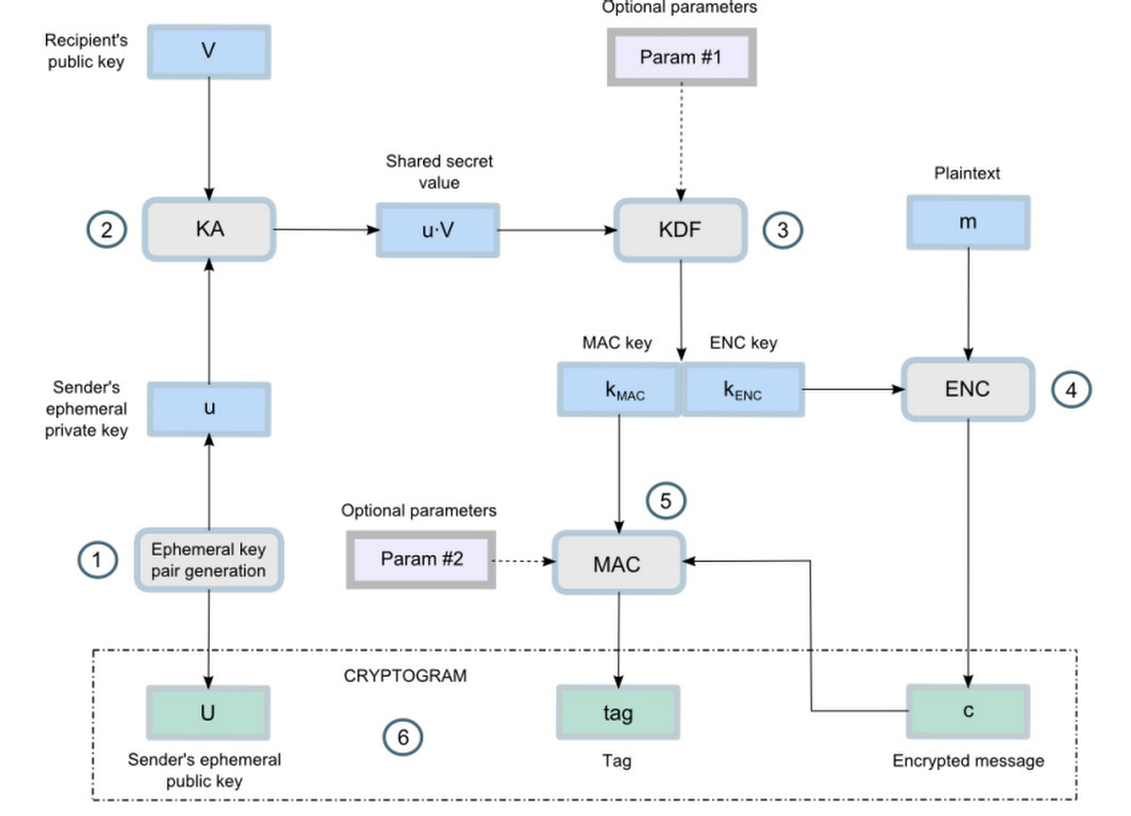
\includegraphics[width=0.5\textwidth]{res/ecies.png}}
    \caption{Ilustrasi proses enkripsi menggunakan ECIES (Sumber: \cite{b7})}
    \label{fig:ecies}
\end{figure}

Pada skema ini, hal yang dilakukan adalah pembangkitan kunci. Ilustrasi dari proses enrkipsi memanfaatkan sistem ini ditunjukan pada Figur \ref{fig:ecies}. Untuk menjelaskan tata cara enkripsi, asumsikan terdapat dua buah pihak yang melakukan komunikasi, yaitu Alice dan Bob. Alice akan mengirimkan pesan $m$ kepada Bob. Proses pembangkitan kunci dilakukan dengan cara sebagai berikut \cite{b2}:

\begin{enumerate}
    \item Alice dan Bob akan menyepakati parameter kurva eliptik yang digunakan. Parameter yang diperlukan adalah $a$, $b$, $p$, dan $G$. Parameter $G$ adalah titik pada kurva eliptik yang digunakan sebagai titik pembangkit (\emph{generator point}).
    \item Bob akan memilih skalar $d_B$ sebagai kunci privatnya.
    \item Bob akan menghitung titik $Q_B = d_B \cdot G$ sebagai kunci publiknya.
    \item Nilai $Q_B$ akan dikirimkan kepada Alice.
\end{enumerate}

Saat Alice menerima nilai $Q_B$, Alice akan melakukan proses enkripsi sebagai berikut:

\begin{enumerate}
    \item Alice memilih skalar $d_A$ sebagai nilai sementara untuk enkripsi.
    \item Alice menghitung titik $Q_m = d_A \cdot G$ sebagai kunci publik sementara.
    \item Alice menghitung \emph{shared key} $K = Q_A + Q_m$.
    \item Alice menghitung kunci enkripsi dan MAC. Hasil dari fungsi KDF ini merupakan konkatenasi dari kunci enkripsi $k_1$ dan kunci MAC $k_2$. 
    \item Alice akan mengenkripsi pesan $m$ menggunakan kunci enkripsi $k_1$. Hasil enkripsi ini disebut dengan $c = E(m, k_1)$.
    \item Hasil enkripsi $c$ akan dihitung nilai MAC-nya menggunakan kunci MAC $k_2$. Hasil dari MAC ini disebut dengan $t = MAC(c, k_2)$.
    \item Alice akan mengirimkan pesan $C = Q_m \parallel c \parallel t$ kepada Bob.
\end{enumerate}

Saat Bob menerima pesan $C$, Bob akan melakukan proses dekripsi sebagai berikut:

\begin{enumerate}
    \item Bob akan memecah terlebih dahulu pesan $C$ menjadi $Q_m$, $c$, dan $t$.
    \item Bob akan menghitung \emph{shared key} $K = Q_m \cdot d_B$.
    \item Bob akan menghitung kunci enkripsi dan MAC. Hasil dari fungsi KDF ini merupakan konkatenasi dari kunci enkripsi $k_1$ dan kunci MAC $k_2$.
    \item Bob akan menghitung nilai MAC dari pesan $c$ menggunakan kunci MAC $k_2$. Hasil dari MAC ini disebut dengan $t' = MAC(c, k_2)$.
    \item Bob akan melakukan verifikasi MAC. Bila $t = t'$, maka pesan $c$ dianggap valid.
    \item Bila pesan $c$ valid, Bob akan mendekripsi pesan $c$ menggunakan kunci enkripsi $k_1$. Hasil dekripsi ini disebut dengan $m = D(c, k_1)$.
\end{enumerate}

Dengan metode seperti itu, pesan $m$ yang dikirimkan oleh Alice dapat dibaca oleh Bob. Selain itu, keunggulan dari metode ini adalah integritas pesan yang dikirimkan dapat diverifikasi. Keunggulan metode ini juga adalah enkripsi dilakukan menggunakan kunci simetris, sehingga proses enkripsi dan dekripsi dapat dilakukan lebih cepat.

\subsection{Tanda Tangan Digital \emph{Elliptic Curve Digital Signature Algorithm} (ECDSA)}

Menurut \cite{b1}, Algoritma ECDSA merupakan algoritma tanda tangan digital yang dikembangkan dari algoritma tanda tangan ElGammal. Algoritma ini dikembangkan oleh Abdala, Bellare, dan Rogaway pada tahun 1999. Asumsikan terdapat dua buah partisipan, yakni Alice dan Bob yang akan melakukan komunikasi. Alice akan mengirimkan pesan $m$ kepada Bob. Alice ingin membuat penjagaan integritas pada pesan $m$ memanfaatkan ECDSA. Proses pembangkitan kunci dilakukan dengan cara sebagai berikut\cite{b2}:

\begin{enumerate}
    \item Alice dan Bob akan menyepakati parameter kurva eliptik yang digunakan. Parameter yang diperlukan adalah $a$, $b$, $p$, dan $G$. Parameter $G$ adalah titik pada kurva eliptik yang digunakan sebagai titik pembangkit (\emph{generator point}).
    \item Alice akan memilih skalar $d_A$ sebagai kunci privatnya.
    \item Alice akan menghitung titik $Q_A = d_A \cdot G$ sebagai kunci publiknya.
    \item Nilai $Q_A$ akan dikirimkan kepada Bob.
    \item Bob akan memilih skalar $d_B$ sebagai kunci privatnya.
    \item Bob akan menghitung titik $Q_B = d_B \cdot G$ sebagai kunci publiknya.
    \item Nilai $Q_B$ akan dikirimkan kepada Alice.
\end{enumerate}

\begin{figure}[htbp]
    \centerline{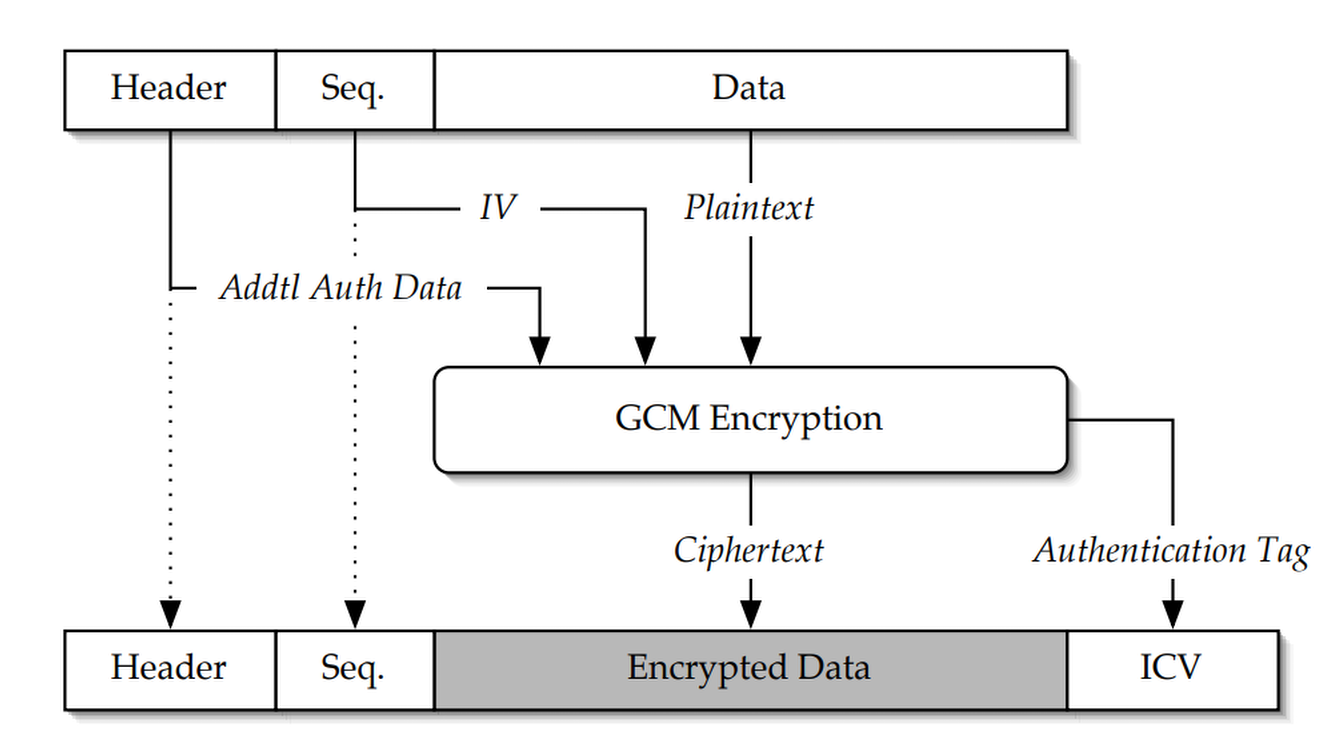
\includegraphics[width=0.5\textwidth]{res/aead.example.png}}
    \caption{Contoh penerapan AEAD pada mode blok GCM. Referensi \cite{b6}}
    \label{fig:aead.example}
\end{figure}

Setelah melakukan pembangkitan kunci, Alice dapat membuat tanda tangan digital pada pesan $m$. Prosedur pembangkitan tanda tangan digital pada pesan $m$ adalah sebagai berikut:

\begin{enumerate}
    \item Alice akan menghitung nilai hash dari pesan $m$. Nilai hash ini disebut dengan $h = H(m)$.
    \item Alice akan memilih skalar $k$ sebagai nilai sementara untuk pembangkitan tanda tangan. Nilai ini harus berada pada rentang $1 \le k < p$.
    \item Alice akan menghitung titik $R = (R_x, R_y) = k \cdot G$. 
    \item Alice akan menghitung nilai $r = x_R \mod p$. Bila $r = 0$, maka Alice akan memilih nilai $k$ yang lain.
    \item Alice akan menghitung nilai $s = k^{-1} \cdot (h + d_A \cdot r) \mod p$. Bila $s = 0$, maka Alice akan memilih nilai $k$ yang lain.
    \item Tanda tangan digital yang dihasilkan adalah pasangan $(r, s)$.
\end{enumerate}

Bob akan melakukan verifikasi tanda tangan digital yang diterima dari Alice. Proses verifikasi tanda tangan digital dilakukan sebagai berikut:

\begin{enumerate}
    \item Bob melakukan verifikasi bahwa nilai $r$ dan $s$ berada pada rentang $1 \le r < n$ dan $1 \le s < n$.
    \item Bob mengambil nilai kunci publik Alice, yakni $Q_A$.
    \item Bob akan menghitung nilai hash dari pesan $m$. Nilai hash ini disebut dengan $h = H(m)$.
    \item Bob akan menghitung nilai $w = s^{-1} \mod p$.
    \item Bob akan menghitung nilai $u_1 = h \cdot w \mod p$ dan $u_2 = r \cdot w \mod p$.
    \item Bob akan menghitung titik $U = u_1 \cdot G + u_2 \cdot Q_A$.
    \item Bila $U = O$, maka tanda tangan digital yang diterima tidak valid. Bila benar, tanda tangan digital yang diterima valid.
\end{enumerate}

Dengan metode seperti itu, Bob dapat memastikan bahwa pesan yang diterima dari Alice tidak diubah oleh pihak lain. Hal ini membuktikan \emph{integrity} dari data tersebut. Selain itu, Bob juga dapat memastikan bahwa pesan tersebut benar-benar berasal dari Alice. Hal ini membuktikan \emph{authenticity} dari pengirim data tersebut.

\subsection{\emph{Authenticated Encryption with Associated Data} (AEAD)}
\label{sec:aead}

Menurut \cite{b4}, AEAD merupakan pengembangan sistem otentikasi pesan terenkripsi yang dilakukan dengan cara yang lebih efisien. Pada AEAD, proses enkripsi serta otentikasi pesan dilakukan dalam satu proses saja. Metode ini merupakan metode yang berbeda bila dibandingkan dengan metode pada umumnya. Sebelum AEAD muncul, proses enkripsi pesan dilakukan dengan melakukan enkripsi pesan terlebih dahulu. Setelah itu, pesan akan diperiksa integritasnya dengan melakukan proses otentikasi. Pada AEAD, proses otentikasi dilakukan pada saat proses enkripsi berlangsung. Salah satu contoh dari enkripsi berbasis AEAD adalah AES dengan mode blok GCM.

Cipher yang menerapkan sistem enkripsi dalam kelas AEAD dapat memiliki \emph{associate data} (AD). Secara desain, data ini tidak dienkripsi, tetapi data ini akan diikutsertakan dalam proses otentikasi yang dihitung bersamaan dengan data yang dienkripsi. Fitur yang ditawarkan pada AEAD ini dapat digunakan untuk menjaga integritas data, seperti untuk menjaga integritas dari \emph{header} pesan. Contoh penerapan AEAD adalah menggunakan blok GCM seperti yang ditunjukan pada figur \ref{fig:aead.example}.


GCM merupakan mode operasi dari enkripsi simetris berbasis blok yang termasuk dalam kelas AEAD. Menurut \cite{b6}, mode ini dapat diimplementasikan sangat baik pada level \emph{hardware} sehingga menghasilkan kecepatan enkripsi yang cepat. Ilustrasi dari proses enkripsi berbasis GCM ditunjukan pada figur \ref{fig1}. Menurut \cite{b6}, terdapat empat input yang dapat terlibat dalam operasi blok GCM. Input tersebut adalah sebagai berikut:

\begin{figure}[htbp]
    \centerline{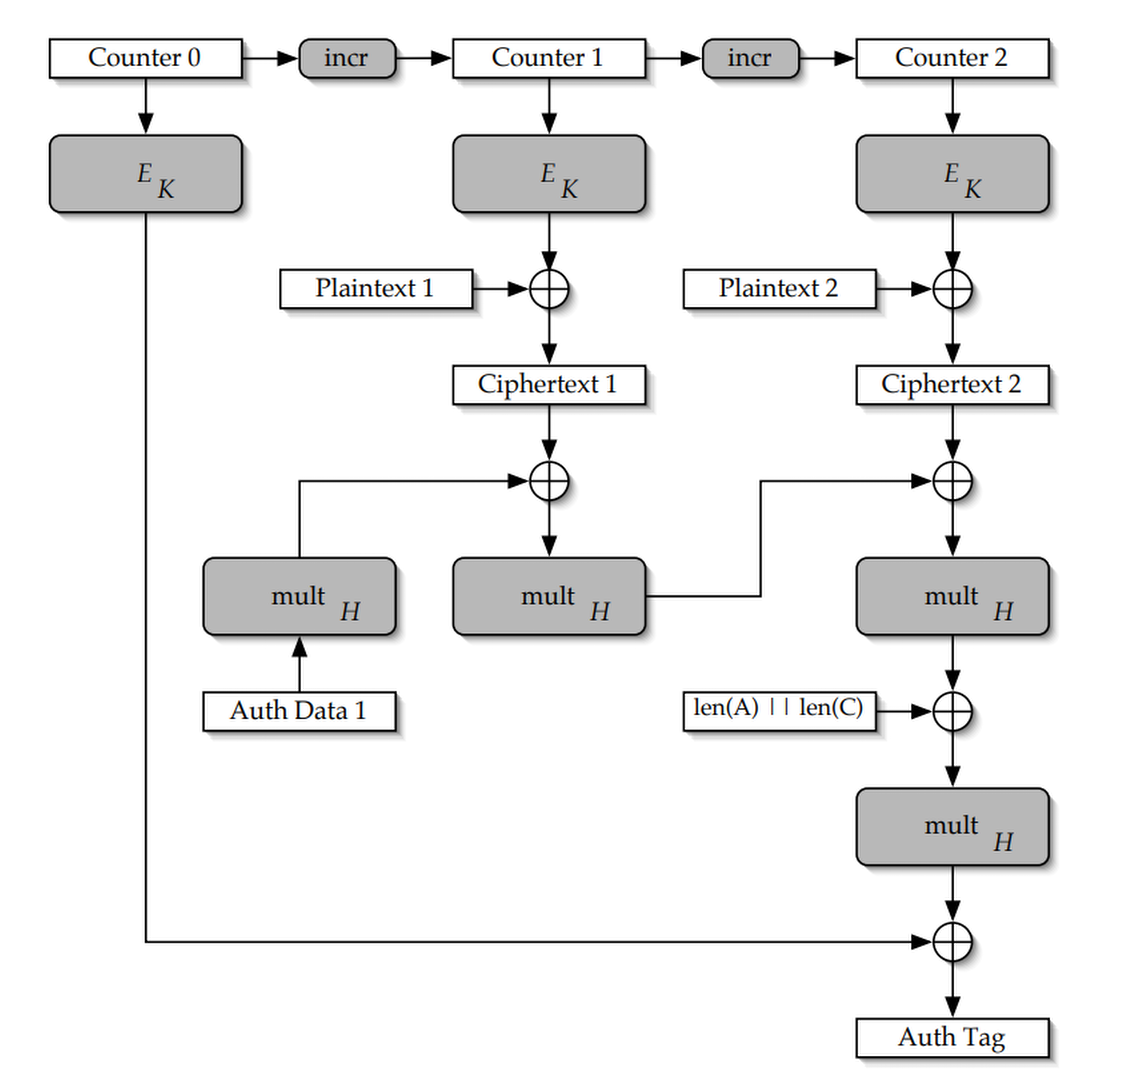
\includegraphics[width=0.5\textwidth]{res/fig1.png}}

    \caption{Ilustrasi proses enkripsi berbasis GCM (Sumber \cite{b6})}
    \label{fig1}
\end{figure}

\begin{enumerate}
    \item \emph{Plaintext}: Pesan yang akan dienkripsi.
    \item \emph{Additional Authenticated Data} (AAD): Data tambahan yang akan diikutsertakan dalam proses otentikasi.
    \item Kunci yang digunakan untuk melakukan enkripsi.
    \item IV \emph{Initialization Vector}: Nilai yang digunakan untuk menginisialisasi counter. Nilai ini juga digunakan untuk menghitung \emph{authentication tag}.
\end{enumerate}

Output dari mode blok ini adalah sebagai berikut:

\begin{enumerate}
    \item \emph{Ciphertext}: Pesan yang telah dienkripsi. Panjang dari \emph{ciphertext} berukuran sama dengan panjang dari \emph{plaintext}.
    \item \emph{Authentication Tag}: Nilai yang digunakan untuk memverifikasi integritas pesan dan AAD.
\end{enumerate}

Metode enkripsi yang dilakukan pada mode GCM pada dasarnya mengikuti proses enkripsi pada mode \emph{counter} (CTR). Proses Enkripsi dilakukan dengan menghitung \emph{counter} untuk blok yang akan dienkripsi. Nilai counter akan dilakukan \emph{increment} dari nilai sebelumnya. Nilai \emph{counter} akan dilakukan proses enkripsi. Hasil enkripsi ini akan dilakukan operasi XOR dengan blok pesan sehingga mendapatkan \emph{ciphertext}. Hasil dari \emph{ciphertext} ini akan diikutsertakan dalam proses otentikasi. Data yang diikutsertakan dalam proses otentikasi adalah \emph{additional data} dan \emph{ciphertext}. Hasil dari otentikasi ini disebut dengan \emph{authentication tag}.

\section{Integrasi Algoritma Enkripsi ECIES dengan Mode Blok GCM}

Berdasarkan bagian \ref{sec:aead}, mode blok berbasis GCM mendukung penggunaan \emph{additional data} (AAD) dalam proses enkripsi. Pada bagian \ref{sec:ecies}, algoritma enkripsi ECIES memerlukan sebuah \emph{authentication tag} untuk memastikan integritas pesan yang dikirimkan. Perhitungan nilai ini pada dasarrnya dapat dilibatkan dengan menambahkan \emph{additional data} pada proses enkripsi menggunakan mode blok GCM. 

\begin{thebibliography}{00}
    \bibitem{b1} Munir, Rinaldi. 2019. Kriptografi. Bandung: Informatika.
    \bibitem{b2} Ali, S., \& Abdul, A. (2016). Data Security for cloud computing based on Elliptic Curve Integrated Encryption Scheme (ECIES) and modified identity based cryptography (MIBC). International Journal of Applied Information Systems, 10(6), 7-13. https://doi.org/10.5120/ijais2016451517.
    \bibitem{b3} Abdalla, M., Bellare, M., \& Rogaway, P. (2021). DHIES: An Encryption Scheme Based on the Diffie-Hellman Problem.
    \bibitem{b4} Rogaway, Phillip. 2002. Authenticated-encryption with Associated-data. In Proceedings of the 9th ACM conference on Computer and communications security (CCS'02). Association for Computing Machinery, New York, NY, USA, 98-107. https://doi.org/10.1145/586110.586125.
    \bibitem{b6} McGrew, D.A., \& Viega, J. (2005). The Galois/Counter Mode of Operation (GCM). https://csrc.nist.rip/groups/ST/toolkit/BCM/documents/proposedmodes/gcm/gcm-spec.pdf.
    \bibitem{b7} Martinez, V. G., Encinas, L. H., \& Ávila, C. S. (2010). A Survey of the Elliptic Curve Integrated Encryption Scheme. Journal of Computer Science and Engineering, 2(2), 7-13. 
\end{thebibliography}

\end{document}
    

% \section{Ease of Use}

% \subsection{Maintaining the Integrity of the Specifications}

% The IEEEtran class file is used to format your paper and style the text. All margins, 
% column widths, line spaces, and text fonts are prescribed; please do not 
% alter them. You may note peculiarities. For example, the head margin
% measures proportionately more than is customary. This measurement 
% and others are deliberate, using specifications that anticipate your paper 
% as one part of the entire proceedings, and not as an independent document. 
% Please do not revise any of the current designations.

% \section{Prepare Your Paper Before Styling}
% Before you begin to format your paper, first write and save the content as a 
% separate text file. Complete all content and organizational editing before 
% formatting. Please note sections \ref{AA}--\ref{SCM} below for more information on 
% proofreading, spelling and grammar.

% Keep your text and graphic files separate until after the text has been 
% formatted and styled. Do not number text heads---{\LaTeX} will do that 
% for you.

% \subsection{Abbreviations and Acronyms}\label{AA}
% Define abbreviations and acronyms the first time they are used in the text, 
% even after they have been defined in the abstract. Abbreviations such as 
% IEEE, SI, MKS, CGS, ac, dc, and rms do not have to be defined. Do not use 
% abbreviations in the title or heads unless they are unavoidable.

% \subsection{Units}
% \begin{itemize}
% \item Use either SI (MKS) or CGS as primary units. (SI units are encouraged.) English units may be used as secondary units (in parentheses). An exception would be the use of English units as identifiers in trade, such as ``3.5-inch disk drive''.
% \item Avoid combining SI and CGS units, such as current in amperes and magnetic field in oersteds. This often leads to confusion because equations do not balance dimensionally. If you must use mixed units, clearly state the units for each quantity that you use in an equation.
% \item Do not mix complete spellings and abbreviations of units: ``Wb/m\textsuperscript{2}'' or ``webers per square meter'', not ``webers/m\textsuperscript{2}''. Spell out units when they appear in text: ``. . . a few henries'', not ``. . . a few H''.
% \item Use a zero before decimal points: ``0.25'', not ``.25''. Use ``cm\textsuperscript{3}'', not ``cc''.)
% \end{itemize}

% \subsection{Equations}
% Number equations consecutively. To make your 
% equations more compact, you may use the solidus (~/~), the exp function, or 
% appropriate exponents. Italicize Roman symbols for quantities and variables, 
% but not Greek symbols. Use a long dash rather than a hyphen for a minus 
% sign. Punctuate equations with commas or periods when they are part of a 
% sentence, as in:
% \begin{equation}
% a+b=\gamma\label{eq}
% \end{equation}

% Be sure that the 
% symbols in your equation have been defined before or immediately following 
% the equation. Use ``\eqref{eq}'', not ``Eq.~\eqref{eq}'' or ``equation \eqref{eq}'', except at 
% the beginning of a sentence: ``Equation \eqref{eq} is . . .''

% \subsection{\LaTeX-Specific Advice}

% Please use ``soft'' (e.g., \verb|\eqref{Eq}|) cross references instead
% of ``hard'' references (e.g., \verb|(1)|). That will make it possible
% to combine sections, add equations, or change the order of figures or
% citations without having to go through the file line by line.

% Please don't use the \verb|{eqnarray}| equation environment. Use
% \verb|{align}| or \verb|{IEEEeqnarray}| instead. The \verb|{eqnarray}|
% environment leaves unsightly spaces around relation symbols.

% Please note that the \verb|{subequations}| environment in {\LaTeX}
% will increment the main equation counter even when there are no
% equation numbers displayed. If you forget that, you might write an
% article in which the equation numbers skip from (17) to (20), causing
% the copy editors to wonder if you've discovered a new method of
% counting.

% {\BibTeX} does not work by magic. It doesn't get the bibliographic
% data from thin air but from .bib files. If you use {\BibTeX} to produce a
% bibliography you must send the .bib files. 

% {\LaTeX} can't read your mind. If you assign the same label to a
% subsubsection and a table, you might find that Table I has been cross
% referenced as Table IV-B3. 

% {\LaTeX} does not have precognitive abilities. If you put a
% \verb|\label| command before the command that updates the counter it's
% supposed to be using, the label will pick up the last counter to be
% cross referenced instead. In particular, a \verb|\label| command
% should not go before the caption of a figure or a table.

% Do not use \verb|\nonumber| inside the \verb|{array}| environment. It
% will not stop equation numbers inside \verb|{array}| (there won't be
% any anyway) and it might stop a wanted equation number in the
% surrounding equation.

% \subsection{Some Common Mistakes}\label{SCM}
% \begin{itemize}
% \item The word ``data'' is plural, not singular.
% \item The subscript for the permeability of vacuum $\mu_{0}$, and other common scientific constants, is zero with subscript formatting, not a lowercase letter ``o''.
% \item In American English, commas, semicolons, periods, question and exclamation marks are located within quotation marks only when a complete thought or name is cited, such as a title or full quotation. When quotation marks are used, instead of a bold or italic typeface, to highlight a word or phrase, punctuation should appear outside of the quotation marks. A parenthetical phrase or statement at the end of a sentence is punctuated outside of the closing parenthesis (like this). (A parenthetical sentence is punctuated within the parentheses.)
% \item A graph within a graph is an ``inset'', not an ``insert''. The word alternatively is preferred to the word ``alternately'' (unless you really mean something that alternates).
% \item Do not use the word ``essentially'' to mean ``approximately'' or ``effectively''.
% \item In your paper title, if the words ``that uses'' can accurately replace the word ``using'', capitalize the ``u''; if not, keep using lower-cased.
% \item Be aware of the different meanings of the homophones ``affect'' and ``effect'', ``complement'' and ``compliment'', ``discreet'' and ``discrete'', ``principal'' and ``principle''.
% \item Do not confuse ``imply'' and ``infer''.
% \item The prefix ``non'' is not a word; it should be joined to the word it modifies, usually without a hyphen.
% \item There is no period after the ``et'' in the Latin abbreviation ``et al.''.
% \item The abbreviation ``i.e.'' means ``that is'', and the abbreviation ``e.g.'' means ``for example''.
% \end{itemize}
% An excellent style manual for science writers is \cite{b7}.

% \subsection{Authors and Affiliations}
% \textbf{The class file is designed for, but not limited to, six authors.} A 
% minimum of one author is required for all conference articles. Author names 
% should be listed starting from left to right and then moving down to the 
% next line. This is the author sequence that will be used in future citations 
% and by indexing services. Names should not be listed in columns nor group by 
% affiliation. Please keep your affiliations as succinct as possible (for 
% example, do not differentiate among departments of the same organization).

% \subsection{Identify the Headings}
% Headings, or heads, are organizational devices that guide the reader through 
% your paper. There are two types: component heads and text heads.

% Component heads identify the different components of your paper and are not 
% topically subordinate to each other. Examples include Acknowledgments and 
% References and, for these, the correct style to use is ``Heading 5''. Use 
% ``figure caption'' for your Figure captions, and ``table head'' for your 
% table title. Run-in heads, such as ``Abstract'', will require you to apply a 
% style (in this case, italic) in addition to the style provided by the drop 
% down menu to differentiate the head from the text.

% Text heads organize the topics on a relational, hierarchical basis. For 
% example, the paper title is the primary text head because all subsequent 
% material relates and elaborates on this one topic. If there are two or more 
% sub-topics, the next level head (uppercase Roman numerals) should be used 
% and, conversely, if there are not at least two sub-topics, then no subheads 
% should be introduced.

% \subsection{Figures and Tables}
% \paragraph{Positioning Figures and Tables} Place figures and tables at the top and 
% bottom of columns. Avoid placing them in the middle of columns. Large 
% figures and tables may span across both columns. Figure captions should be 
% below the figures; table heads should appear above the tables. Insert 
% figures and tables after they are cited in the text. Use the abbreviation 
% ``Fig.~\ref{fig}'', even at the beginning of a sentence.

% \begin{table}[htbp]
% \caption{Table Type Styles}
% \begin{center}
% \begin{tabular}{|c|c|c|c|}
% \hline
% \textbf{Table}&\multicolumn{3}{|c|}{\textbf{Table Column Head}} \\
% \cline{2-4} 
% \textbf{Head} & \textbf{\textit{Table column subhead}}& \textbf{\textit{Subhead}}& \textbf{\textit{Subhead}} \\
% \hline
% copy& More table copy$^{\mathrm{a}}$& &  \\
% \hline
% \multicolumn{4}{l}{$^{\mathrm{a}}$Sample of a Table footnote.}
% \end{tabular}
% \label{tab1}
% \end{center}
% \end{table}

% \begin{figure}[htbp]
% \centerline{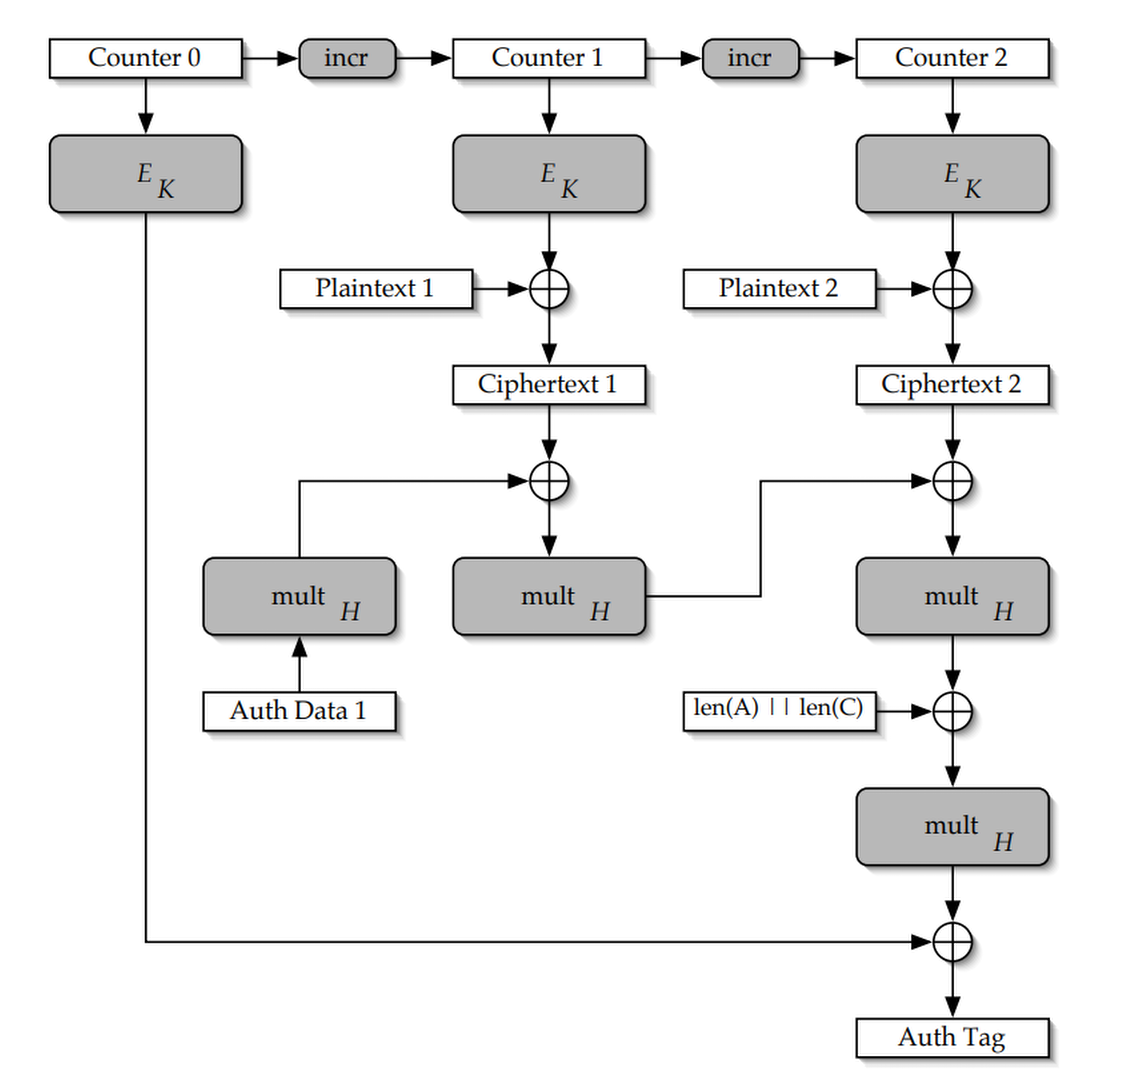
\includegraphics{res/fig1.png}}
% \caption{Example of a figure caption.}
% \label{fig}
% \end{figure}

% Figure Labels: Use 8 point Times New Roman for Figure labels. Use words 
% rather than symbols or abbreviations when writing Figure axis labels to 
% avoid confusing the reader. As an example, write the quantity 
% ``Magnetization'', or ``Magnetization, M'', not just ``M''. If including 
% units in the label, present them within parentheses. Do not label axes only 
% with units. In the example, write ``Magnetization (A/m)'' or ``Magnetization 
% \{A[m(1)]\}'', not just ``A/m''. Do not label axes with a ratio of 
% quantities and units. For example, write ``Temperature (K)'', not 
% ``Temperature/K''.

% \section*{Acknowledgment}

% The preferred spelling of the word ``acknowledgment'' in America is without 
% an ``e'' after the ``g''. Avoid the stilted expression ``one of us (R. B. 
% G.) thanks $\ldots$''. Instead, try ``R. B. G. thanks$\ldots$''. Put sponsor 
% acknowledgments in the unnumbered footnote on the first page.

% \section*{References}

% Please number citations consecutively within brackets \cite{b1}. The 
% sentence punctuation follows the bracket \cite{b2}. Refer simply to the reference 
% number, as in \cite{b3}---do not use ``Ref. \cite{b3}'' or ``reference \cite{b3}'' except at 
% the beginning of a sentence: ``Reference \cite{b3} was the first $\ldots$''

% Number footnotes separately in superscripts. Place the actual footnote at 
% the bottom of the column in which it was cited. Do not put footnotes in the 
% abstract or reference list. Use letters for table footnotes.

% Unless there are six authors or more give all authors' names; do not use 
% ``et al.''. Papers that have not been published, even if they have been 
% submitted for publication, should be cited as ``unpublished'' \cite{b4}. Papers 
% that have been accepted for publication should be cited as ``in press'' \cite{b5}. 
% Capitalize only the first word in a paper title, except for proper nouns and 
% element symbols.

% For papers published in translation journals, please give the English 
% citation first, followed by the original foreign-language citation \cite{b6}.

